\subsection{Intuition with Geometry}
Which is more symmetrical, a scalene triangle or an equilateral triangle? Clearly, the equilateral triangle has more symmetries; you can rotate it $120\degree$ or $240\degree$, and you can reflect it across three axes. The scalene triangle has no symmetries that modify the object, but by convention we call the `do-nothing' operation a symmetry as well.

By a `symmetry' of an object, we mean something that we can do to it that preserves its structure. In the case of these shapes, we want to preserve the vertices and edges; these symmetries are rotations and reflections. For the equilateral triangle then, what are all the symmetries?

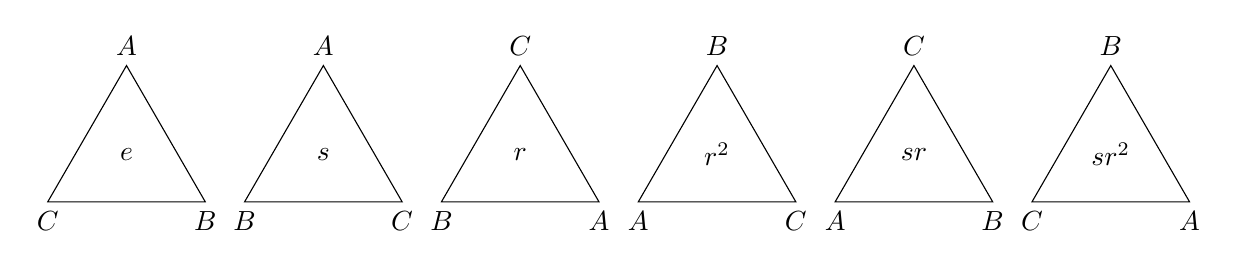
\begin{tikzpicture}
	\draw (0,0) node[below]{$C$}
	-- (2,0) node[below]{$B$}
	-- (1,1.73) node[above]{$A$}
	-- cycle;
	\draw(1, 0.6) node{$e$};

	\draw (2.5,0) node[below]{$B$}
	-- (4.5,0) node[below]{$C$}
	-- (3.5,1.73) node[above]{$A$}
	-- cycle;
	\draw(3.5, 0.6) node{$s$};

	\draw (5,0) node[below]{$B$}
	-- (7,0) node[below]{$A$}
	-- (6,1.73) node[above]{$C$}
	-- cycle;
	\draw(6, 0.6) node{$r$};

	\draw (7.5,0) node[below]{$A$}
	-- (9.5,0) node[below]{$C$}
	-- (8.5,1.73) node[above]{$B$}
	-- cycle;
	\draw(8.5, 0.6) node{$r^2$};

	\draw (10,0) node[below]{$A$}
	-- (12,0) node[below]{$B$}
	-- (11,1.73) node[above]{$C$}
	-- cycle;
	\draw(11, 0.6) node{$sr$};

	\draw (12.5,0) node[below]{$C$}
	-- (14.5,0) node[below]{$A$}
	-- (13.5,1.73) node[above]{$B$}
	-- cycle;
	\draw(13.5, 0.6) node{$sr^2$};
\end{tikzpicture}

As stated before, we assign the letter $e$ to the identity element. The operation $s$ is a reflection; $r$ is a rotation. By combining these elements, we get the set of elements of the group. Note that order matters: $sr\neq rs$.

\subsection{Basic Notion}
\begin{definition}[Group]
	A group is a set $G$ together with a way of composing its elements $\ast$ satisfying ($\forall g, h, k \in G$):
	\begin{itemize}
		\item (closure) $g \ast h \in G$
		\item (identity) $\exists e \in G \mathrm{\ s.t.\ } e \ast g = g \ast e = g$
		\item (inverses) $\exists g^{-1} \in G \mathrm{\ s.t.\ } g \ast g^{-1} = g^{-1} \ast g = e$
		\item (associativity) $g \ast (h \ast k) = (g \ast h) \ast k$
	\end{itemize}
\end{definition}

Formally, we might say that a set $G$ with a binary operation $\ast : G \times G \to G$ is a group if it follows the last three axioms; the first rule is implicit in the function's type.

\subsection{Examples}
\begin{enumerate}
	\setcounter{enumi}{-1}
	\item $G = \{ e \}$ --- this is the `trivial group'.
	\item $G = \{ \text{symmetries of the equilateral triangle} \} $; $\ast$ is defined by: `$g \ast h$ means doing $h$ then $g$'.
	\item $G = (\mathbb Z, +)$. This is easy to prove by verifying the axioms.
	\item $G = (\mathbb R, +); (\mathbb Q, +); (\mathbb C, +)$
	\item $G = (\mathbb R^*, \cdot)$ where $\mathbb R^* = \mathbb R \setminus \{ 0\}$. Note that $(\mathbb R, \cdot)$ is not a group, because $\nexists 0^{-1} \in \mathbb R \st 0^{-1} \cdot 0 = 0 \cdot 0^{-1} = 1$.
	\item $G = (\mathbb R, \ast)$ where $r \ast s := r + s + 5$.
	\item $G = (\mathbb Z_n, +)$ where $\mathbb Z_n = \{ 0, 1, 2, \cdots, n-1 \}$ and addition is done modulo $n$.
	\item A vector space with the operation of vector addition is a group.
	\item $GL_2(\mathbb R)$ is the set of invertible $2\times 2$ matrices, which is a group with respect to matrix multiplication.
\end{enumerate}

\subsection{Non-Examples}
\begin{enumerate}
	\item $G = (\mathbb Z_n, +)$ where addition is not performed modulo $n$. This group is not closed, e.g. $(n-1) + 2 \notin G$.
	\item $G = (\mathbb Z, \cdot)$ because $\nexists n\in \mathbb Z \st 2 \cdot n = n \cdot 2 = 1$.
	\item $G = (\mathbb R, \ast)$ where $r \ast s = r^2 s$ because there is no identity element.
	\item $G = (\mathbb N, \ast)$ where $n \ast m := \abs{n - m}$ because it is non-associative, e.g. $1 \ast (2 \ast 5) = 2$; $(1 \ast 2) \ast 5 = 4$.
\end{enumerate}
